\chapter{Detecting crucial parts in inputs}
\label{inputReduction:intro}
When we detect that the program under test (PUT) crashes, wrongly satisfied, wrongly unsatisfied, hangs or gives the wrong solution on a given input we want to know why it does that. What causes this unwanted output and on what line does the bug occurs. 
With crashes, a stack trace and some luck this could be easy, but when a bug causes a crash in another place the developer may need to debug deep into the code to find the bug. 
This with potential large inputs could be a tedious and long assignment, for this reason we would like to know what parts of the input are relevant for the bug. We will discover this further in this chapter, starting with deobfuscating inputs.


\section{Deobfuscating inputs}
\label{inputReduction:Deobfuscating}
\begin{quote}
	"Often people who encounter a bug spend a lot of time investigating which changes to the input file will make the bug go away and which changes will not affect it." 
	\newline
	-Richard Stallman and Ralf Hildebrandt in "Simplifying and Isolating Failure-Inducing Input" \cite{5zeller2002simplifyingIsolatingFailure-inducing}.
\end{quote} 
When receiving a big input, the chance of it having parts unrelated to the bug is almost guaranteed, we will call these inputs (unintentionally) obfuscated inputs. Deobfuscating those inputs can take a lot of try and error to see which variations still reveal the bug or having to walk through the execution to find the bug. Both take a while if we want to go to absolute minimal inputs, but for developers it is not needed to go to that extreme. As long as we take the bulk of the unrelated parts of inputs are gone it will help the developer to find the bug faster. With these techniques we can also group similar bugs and duplicate errors (more on that later) which is also useful information for developers. To find crucial parts of inputs, it is often achieved either with simplification or isolation. 

\subsection{Simplifying}
\label{inputReduction:Simplifying}
Simplification is the technique where we repeatably remove parts of a failing input and check if it still fails and it often done via a "delta-debugging" algorithm, which belongs to the divide-and-conquer family of algorithms \cite{2FuzzingAndDeltaDebuggingSMTSolvers}. 
The algorithm can be seen in figure \ref{fig:ddmin} with 
"$ c_{\mbox{\ding{56}}} $"  %c_X
meaning the failing input to be deobfuscated,
"\ding{52}" %checkmark 
meaning that a test passed with the given input,
"\ding{56}" %cross 
failed with the given input, 
"$\Delta$" and "$\nabla$" being a subset of the input and the complement of the former and
"1-minimal" meaning that not a single character can change without the input going from failing to passing. Firstly, we start the algorithm with the input and a split "n" of two. If we can find a subset that still fails on its own, then we continue with that subset else we look for a subset where the complement of the input still fails but where a subset is missing from the input. In the case where we split the input in two parts this would be the same as the previous. In case we do not find any smaller subset to continue, then we reduce de granularity of the split by two. To finally end when it is no longer possible to remove any part of the input, we then have obtained an input where all parts are necessary to expose the bug. This input is at the same time also the shortest possible input to trigger this bug making finding the bug for the developer easier than in the original input filled with unrelated parts. 
An example of delta-debugging to minimize input can be found in figure \ref{fig:ddminExample}. In the first two steps no removal of any part nor complement was possible therefore we reduce the granularity, after which a removal of parts 3 and 4 was found possible. To then use some previous knowledge (lines 9, 10 and 11) with 2 new tests to remove parts 5 and 6. To then decrease the granularity again, repeat our possible steps and reach a minimal input.

\begin{figure}
	\centering
	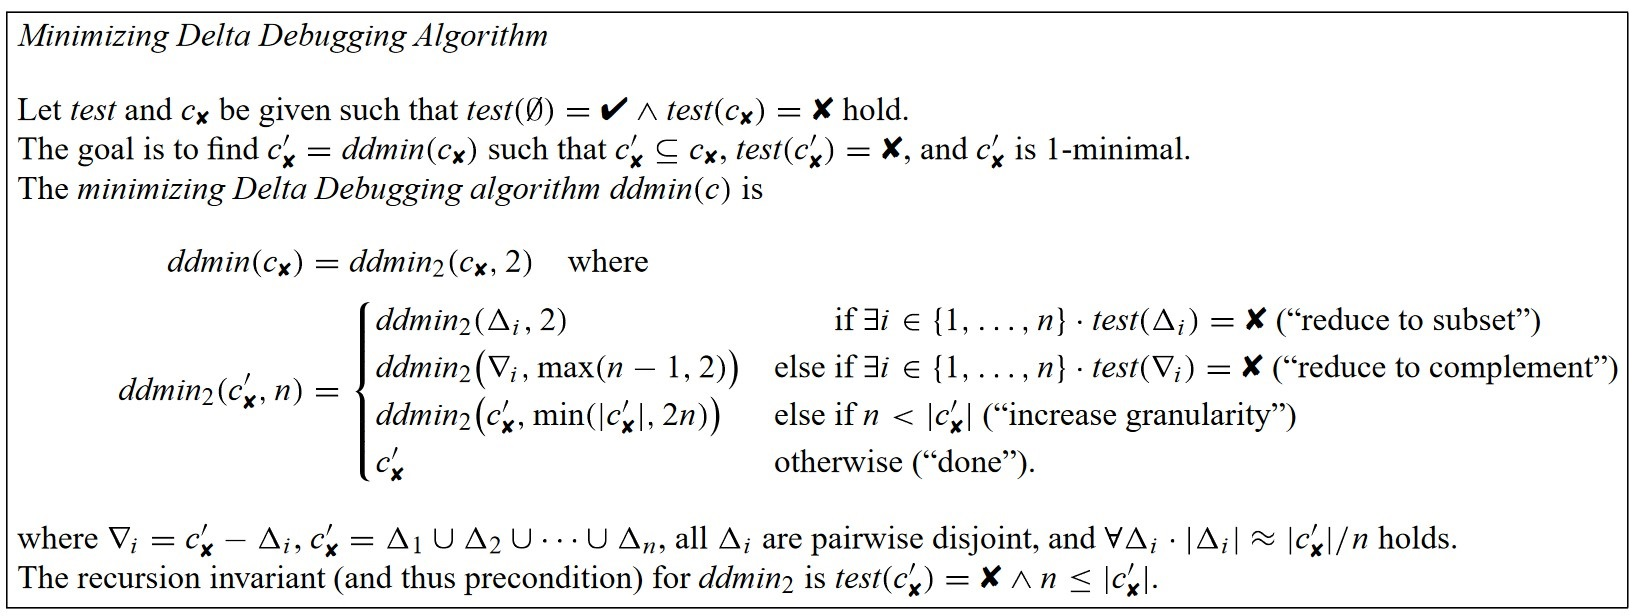
\includegraphics[width=1.0\textwidth]{images/ddminFromPaper5edit}
	\caption{A minimizing delta-debugging algorithm as shown in "Simplifying and isolating failure-inducing input" by Andreas Zeller and Ralf Hildebrandt \cite{5zeller2002simplifyingIsolatingFailure-inducing}.}
	\label{fig:ddmin}
\end{figure}

\begin{figure}
	\centering
	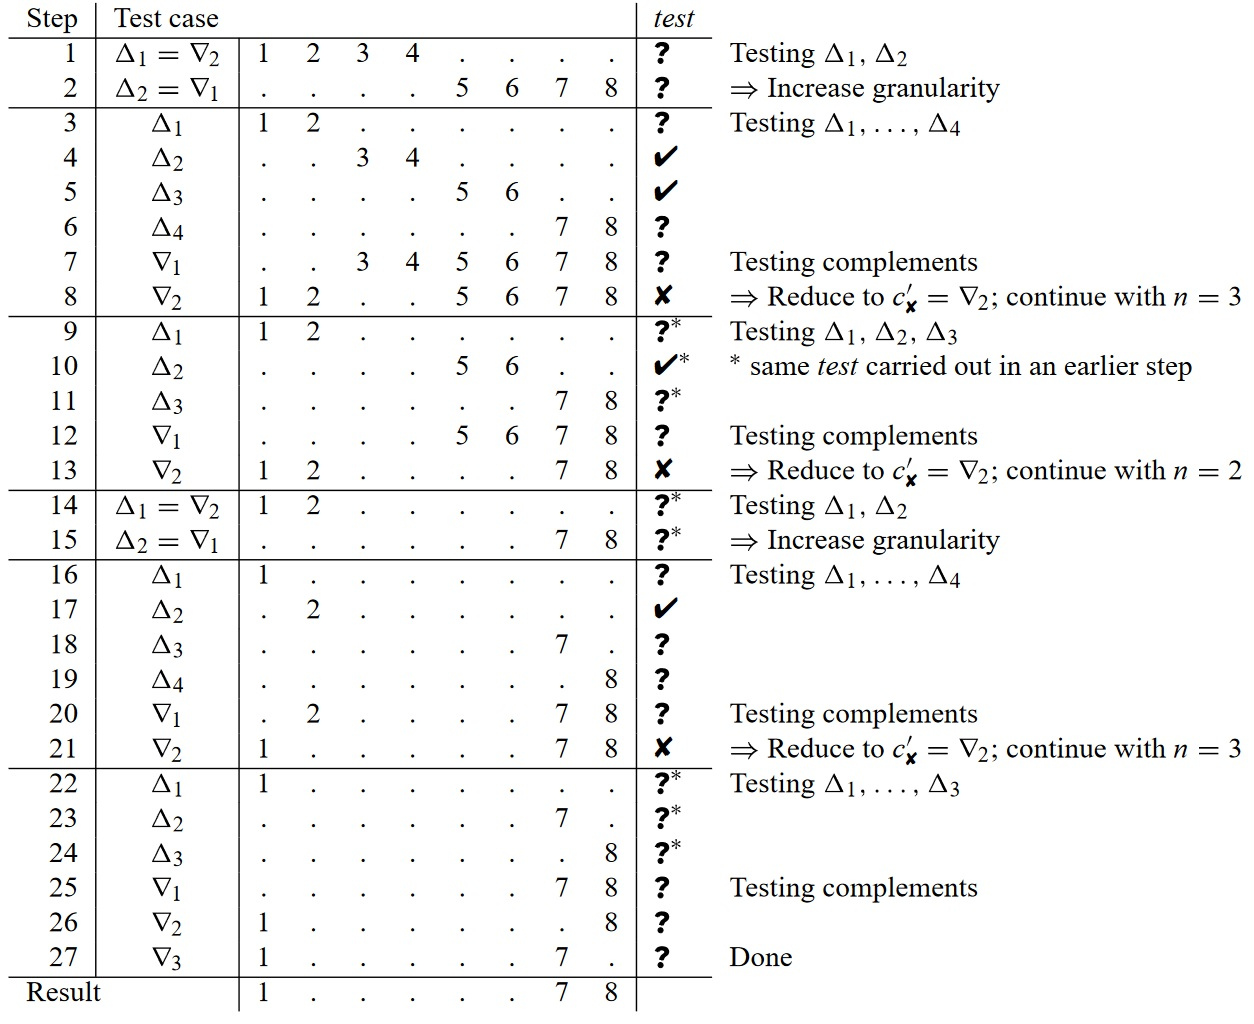
\includegraphics[width=1.0\textwidth]{images/ddminExampleFromPaper5}
	\caption{A minimizing delta-debugging example as shown in "Simplifying and isolating failure-inducing input" by Andreas Zeller and Ralf Hildebrandt \cite{5zeller2002simplifyingIsolatingFailure-inducing} with an input that is deobfuscated with the ddmin() algorithm from figure \ref{fig:ddmin}.}
	\label{fig:ddminExample}
\end{figure}

\subsection{Isolation}
\label{inputReduction:Isolation}
The second technique, isolation, is a technique where instead of minimizing the input we try to find the smallest difference between an input that shows the bug versus an input that does not show the bug. This comes with the advantage that no matter if we find the bug or not the difference will diminish, either the maximum input will shrink or the minimum input will grow. 
This technique brings extra complexity with the tracking of multiple inputs and bigger inputs often take longer to process, but according to Andreas Zeller et al. \cite{5zeller2002simplifyingIsolatingFailure-inducing} this is the faster one to the two techniques. 
Figure \ref{fig:simplificationIsolation} shows the difference between simplifying and isolation both finding the critical part of the input. With simplification the critical part is indicated by the last test in the figure while with isolation it is the difference of the last passed and last failed tests. And the '*' indicates that the result is already known and does not need to be recalculated.
\begin{figure}
	\centering
	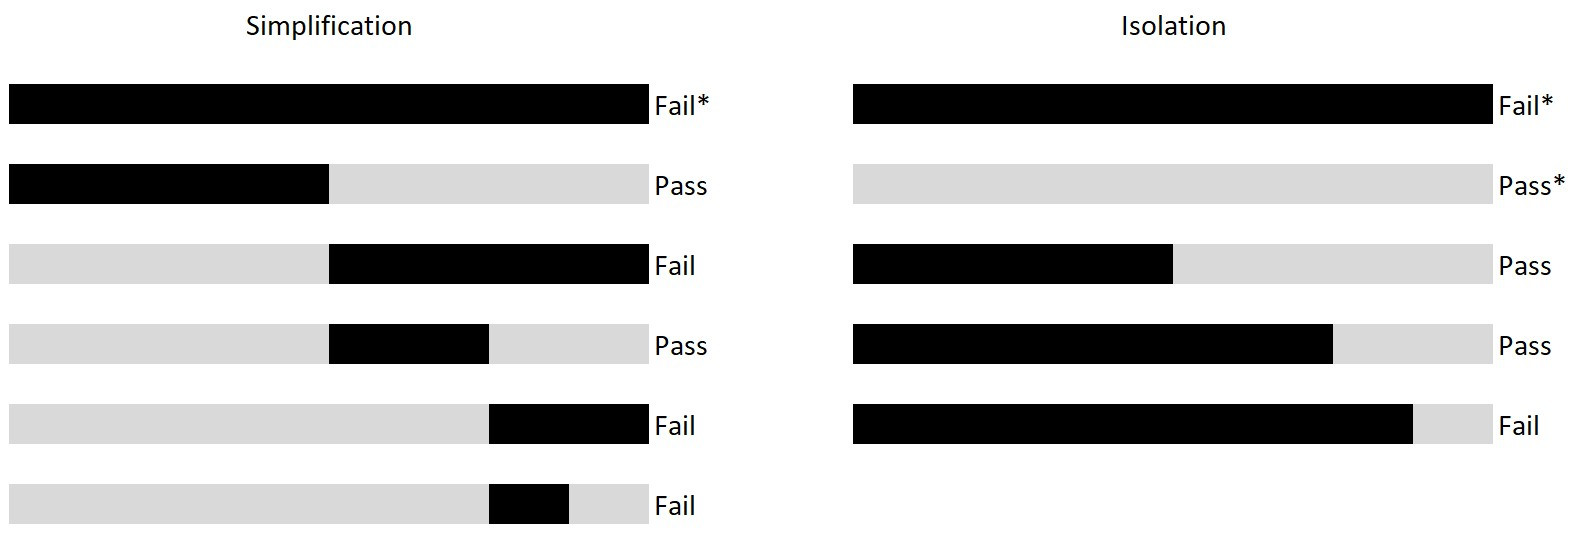
\includegraphics[width=1.0\textwidth]{images/simplificationIsolation}
	\caption{Deobfuscating inputs based on simplification (left) and isolation (right) on the same input. Figure based on an illustration found in "Why programs fail: a guide to systematic debugging" by Andreas Zeller \cite{bookZellerwhyProgramsFail}.}
	\label{fig:simplificationIsolation}
\end{figure}

\subsection{Connection with minimal unsatisfiable subset and maximally satisfiable subsets}
\label{inputReduction:MUS/MSS}
For readers that are familiar with the SMT of constraint solving-world will have noticed that this techniques feels similar to a way of finding the minimal unsatisfiable subset (MUS), which it is in the case of a solver wrongly stating that an input is unsatisfiable. 
With MUS you try to find the smallest subset of formulas or constraints that will result in an unsatisfiable solution while with 
MSS you would be trying to find the biggest subset of formulas or constraints that would result in a satisfiable solution. Both are an iterative process and can be applied in the simplification or the isolation process. But solving which combination of formulas results in the smallest of biggest subset is a computationally intensive progress. Fortunately, a lot of thought has already been put in it to improve it, for example Mark H. Liffiton et al. have proposed multiple "Algorithms for Computing minimal unsatisfiable subsets of Constraints" \cite{51liffiton2008algorithms}. In which they discuss their novel sound and complete algorithms for finding all minimal unsatisfiable subsets. Again, we should note that a minimal input is not needed as we aim to reduces de input to help de developer find the error faster, a difference between a smaller and the absolute minimum will cause for a big computational difference in practice.

\subsection{Alternative approach}
\label{inputReduction:alt2deobfuscating}
An alternative approach compared to the already mentioned techniques is one by Alexandra Bugariu and Peter M\"uller \cite{9bugariu2020automaticallyTestingStringSolvers}. In which they forgo the need of deobfuscating inputs by generating inputs "small by construction". 
Because the smaller the inputs are the less space there is for remaining stuff to obfuscate the input. On the other hand, the chance of finding bigger bugs with multiple constraints interacting with each other will become harder.
A last alternative approach would be retrying fuzzing the same seed after that seed has produced an unwanted input with adding an increasing size limitation in order to find the same bug with a smaller input as done by Muhammad Numair Mansur et al. in "Detecting Critical Bugs in SMT Solvers Using Blackbox Mutational Fuzzing" \cite{1mansur2020detecting}.

\section{What size to change}
\label{inputReduction:Chucksize}
A subject we glossed over so far is the chuck size, the size to remove while trying to find the critical parts of the inputs. 
The previous seen techniques will work well on the original fuzz testing by Miller et al. \cite{4originalFuzzingUnixUtils} since those random generated symbols where independent from each other. But when testing more complex words such as function names, we no longer can split on all possible places, since the input would most likely no longer parse. 
In figure \ref{fig:simplificationIsolation} we conveniently took one-eighth of the input as the chuck sizes for the ease of the example. For performance reasons we hope we can keep our chuck sizes as big as possible to be able to discard larger unrelated parts of the inputs. But when this is not possible, we will need to decrease the granularity of the chuck sizes.
For example, to be able to find the critical parts of an input of the form "XXooXooXXoo" (with 'o' being the critical parts and the 'X' being unrelated to the bug) we should always search further with same granularity while the removed parts are already removed until all options with that granularity are searched \cite{bookZellerwhyProgramsFail}. This will make sure that we eliminate all unrelated parts with the specific granularity and get "ooXoooo" instead of "ooXooXXoo". 

For more complex inputs we can apply techniques seen in section \ref{fuzzing:InputStructure} where we discussed the creation of randomly and smarter created inputs. Instead of removing unrelated parts based purely on where the part sits in the input, we can use knowledge of the input structure or knowledge of the PUT to guide us in the removal \cite{bookZellerwhyProgramsFail}. Both lexical (the meaning of words) and syntactical knowledge (the meaning of word combinations) can be used to help us in deobfuscating complex inputs. Where syntactical knowledge would help us remove the most since it is the bigger of the two.

\subsection{Preserving satisfiability}
\label{inputReduction:preservingSat}
With the techniques as mentioned in section \ref{fuzzing:handelingOracelproblem}, "satisfiable by construction" formed inputs will need to take the extra complexity of preserving the ground truth in mind when deobfuscating inputs. When the ground truth says that an input should be unsatisfiable and the PUT says it is a satisfiable problem with the following output, then we cannot remove constraints to retest if that specific constraint was the cause without knowing the new ground truth. As potential change could switch the original input from an unsatisfiable to a satisfiable problem. We could use a trusted solver to make sure that we do not change the ground truth by retesting each change as Brummayer and Biere \cite{2FuzzingAndDeltaDebuggingSMTSolvers} did.
Or as done by  Muhammad Numair Mansur et al. \cite{1mansur2020detecting} try to fuzz the same seed in the hope to find a smaller input that gives the same bug. 
In the other scenario when he ground truth says that an input should be satisfiable with X amount of models and the PUT says that the input is unsatisfiable. Then we have more options to deobfuscate the inputs. We can use the previously mentioned techniques such as simplifying, isolation, MUS, MSS and the technique of re-fuzzing such as STORM did, while still preserving the (un)satisfiability of the problem.

\section{Unexpected advantages of deobfuscation}
\subsection{Deduplication}
\label{inputReduction:Deduplication}
With deobfuscating the inputs, we can detect exact copies, but depending on the deobfuscation's time complexity other techniques could be better with similar results. In case where we would have access to stack traces, we could differentiate the bugs on the basis of the hash from the backtrace, sometimes even numerous hashes per input depending on the number of backtrace lines taken to hash. This technique is called "stack backtrace hashing" and is quite popular according to Valentin J.M. Man\`es et al. \cite{13manes2019survey}.
Another technique talked about in that paper, is looking at the code coverage generated by the inputs where the executed path (or hash of it) is used as a fingerprint of the inputs. A technique, used by Microsoft \cite{36semanticsAwareDeduplicationRETracer} is called "semantics based deduplication", where instead of backtrace they use memory dumps to hopefully find the origins of bugs. This use of dumps is less ideal due to traces having more information, but the latter is not always possible due to traces often being removed in production for performance and privacy reasons as specified in the paper. 
A last technique would be looking at the bug description left by manual user bug reports, although this dependence on the quality of bug reports and is most likely poorly automatable.
None of the techniques mentioned above are perfect: with stack backtrace hashing you need access to the backtrace, with coverage some inputs will generate extra function calls and the semantics based deduplication are limited to X86 or x86-64 code with the binary file and the debug information. Neither of those first techniques will work with black box fuzzing unfortunately due to the limited information given as output.

\subsection{The precision effect}
\label{inputReduction:PersisionEffect}
The finding of the same bug needs to be done carefully, so that we do not change a null pointer dereference bug to a parser related bug. This, as discussed in the previous chapter, is because we value some bugs higher than others. 
In a paper by Andreas Zeller and Ralf Hildebrandt \cite{5zeller2002simplifyingIsolatingFailure-inducing} they talk about this exact problem which they called "the Precision Effect". Sometimes this is not a problem, for example when we are trying to find all possible bugs and will rerun the fuzzer after each incremental improvement or the situation where a deeper bug turns into another deep bug. But overall, we try to avoid this effect, which can be done with the techniques in the previous section. But compared to the previous section where we try to match bugs here, we try to detect if we get the same bug as the last time.

\section{Conclusion}
\label{inputReduction:Conclusion}
In this chapter we discussed why a deobfuscated input would be convenient for the further process, what advantages it brings with it while fuzzing PUTs. We have seen multiple methods of deobfuscating inputs from the straightforward simplifying to the heavier isolation. We also looked at state-of-the-art approaches, how they preserve satisfiability and how to avoid having to deobfuscate inputs in the first place. To then end with more advantages of deobfuscated inputs.

%%% Local Variables: 
%%% mode: latex
%%% TeX-master: "thesis"
%%% End: 
